\documentclass[tikz,border=5mm]{standalone}
\usepackage{tikz}
\usetikzlibrary{calc}

\begin{document}
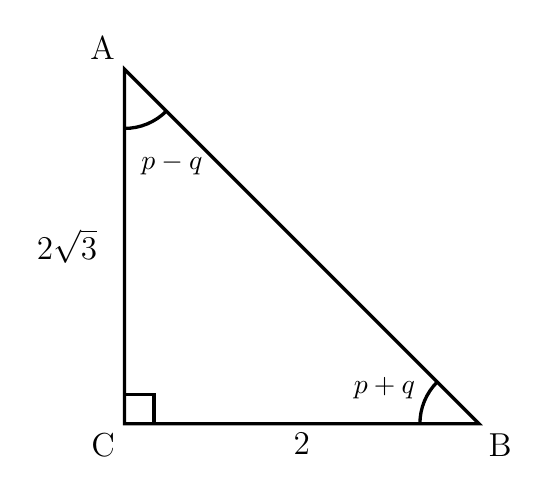
\begin{tikzpicture}[scale=1.5]

% Define coordinates
\coordinate (A) at (0,3);
\coordinate (C) at (0,0);
\coordinate (B) at (3,0);

% Draw triangle
\draw[very thick] (A) -- (C) -- (B) -- cycle;

% Right angle mark at C
\draw[very thick] (C) rectangle ++(0.25,0.25);

% Angle arc at A (p-q)
\draw[very thick] ($(A)!0.5cm!(C)$) arc[start angle=-90, end angle=-45, radius=0.5cm];
\node at ($(A)+(0.4,-0.8)$) {$p-q$};

% Angle arc at B (p+q)
\draw[very thick] ($(B)!0.5cm!(C)$) arc[start angle=180, end angle=135, radius=0.5cm];
\node at ($(B)+(-0.80,0.3)$) {$p+q$};

% Labels for vertices
\node[above left] at (A) {\large A};
\node[below left] at (C) {\large C};
\node[below right] at (B) {\large B};

% Labels for sides
\node[left] at ($(A)!0.5!(C)+(-0.15,0)$) {\large $2\sqrt{3}$};
\node[below] at ($(C)!0.5!(B)$) {\large $2$};

\end{tikzpicture}
\end{document}